\section{Material and Methods} \label{matmet}

\subsection{Data}

\subsection{Preprocessing}

\gls{eeg} and \gls{emg} signals were resampled from approximately 200.0Hz to 256.0Hz using
conservative sinc interpolation\citationneeded{Putman}.
A Frequency of 256.0Hz is convenient since is implies that discrete wavelet decomposition (see subsection~\ref{sub:features} and fig.~\ref{fig:dwd}) will separate
frequencies above 4.0Hz from those below 4.0Hz (since $4 = 256.0/{2^6} $).
This frequency is typically uses as a cut-off value between theta and delta waves \citationneeded{}.
In addition, \gls{eeg} and \gls{emg} signals were standardised ($E[x] = 0, Var[x] = 1$) to account for the variability in baseline amplitude due to acquisition.
Annotations labels were resampled at exactly 0.20Hz using nearest neighbour interpolation.

\subsection{Feature extraction}
\label{sub:features}

A wavelet transform based feature extraction strategy was adopted.
In summary, discrete wavelet decomposition was used on \gls{eeg} and \gls{emg}
in order to separate frequency bands (fig.~\ref{fig:dwd}).
Then all features were computed on five second epochs for all wavelet coefficients as well as raw signals.

\begin{figure}[h!]
  \centering   
    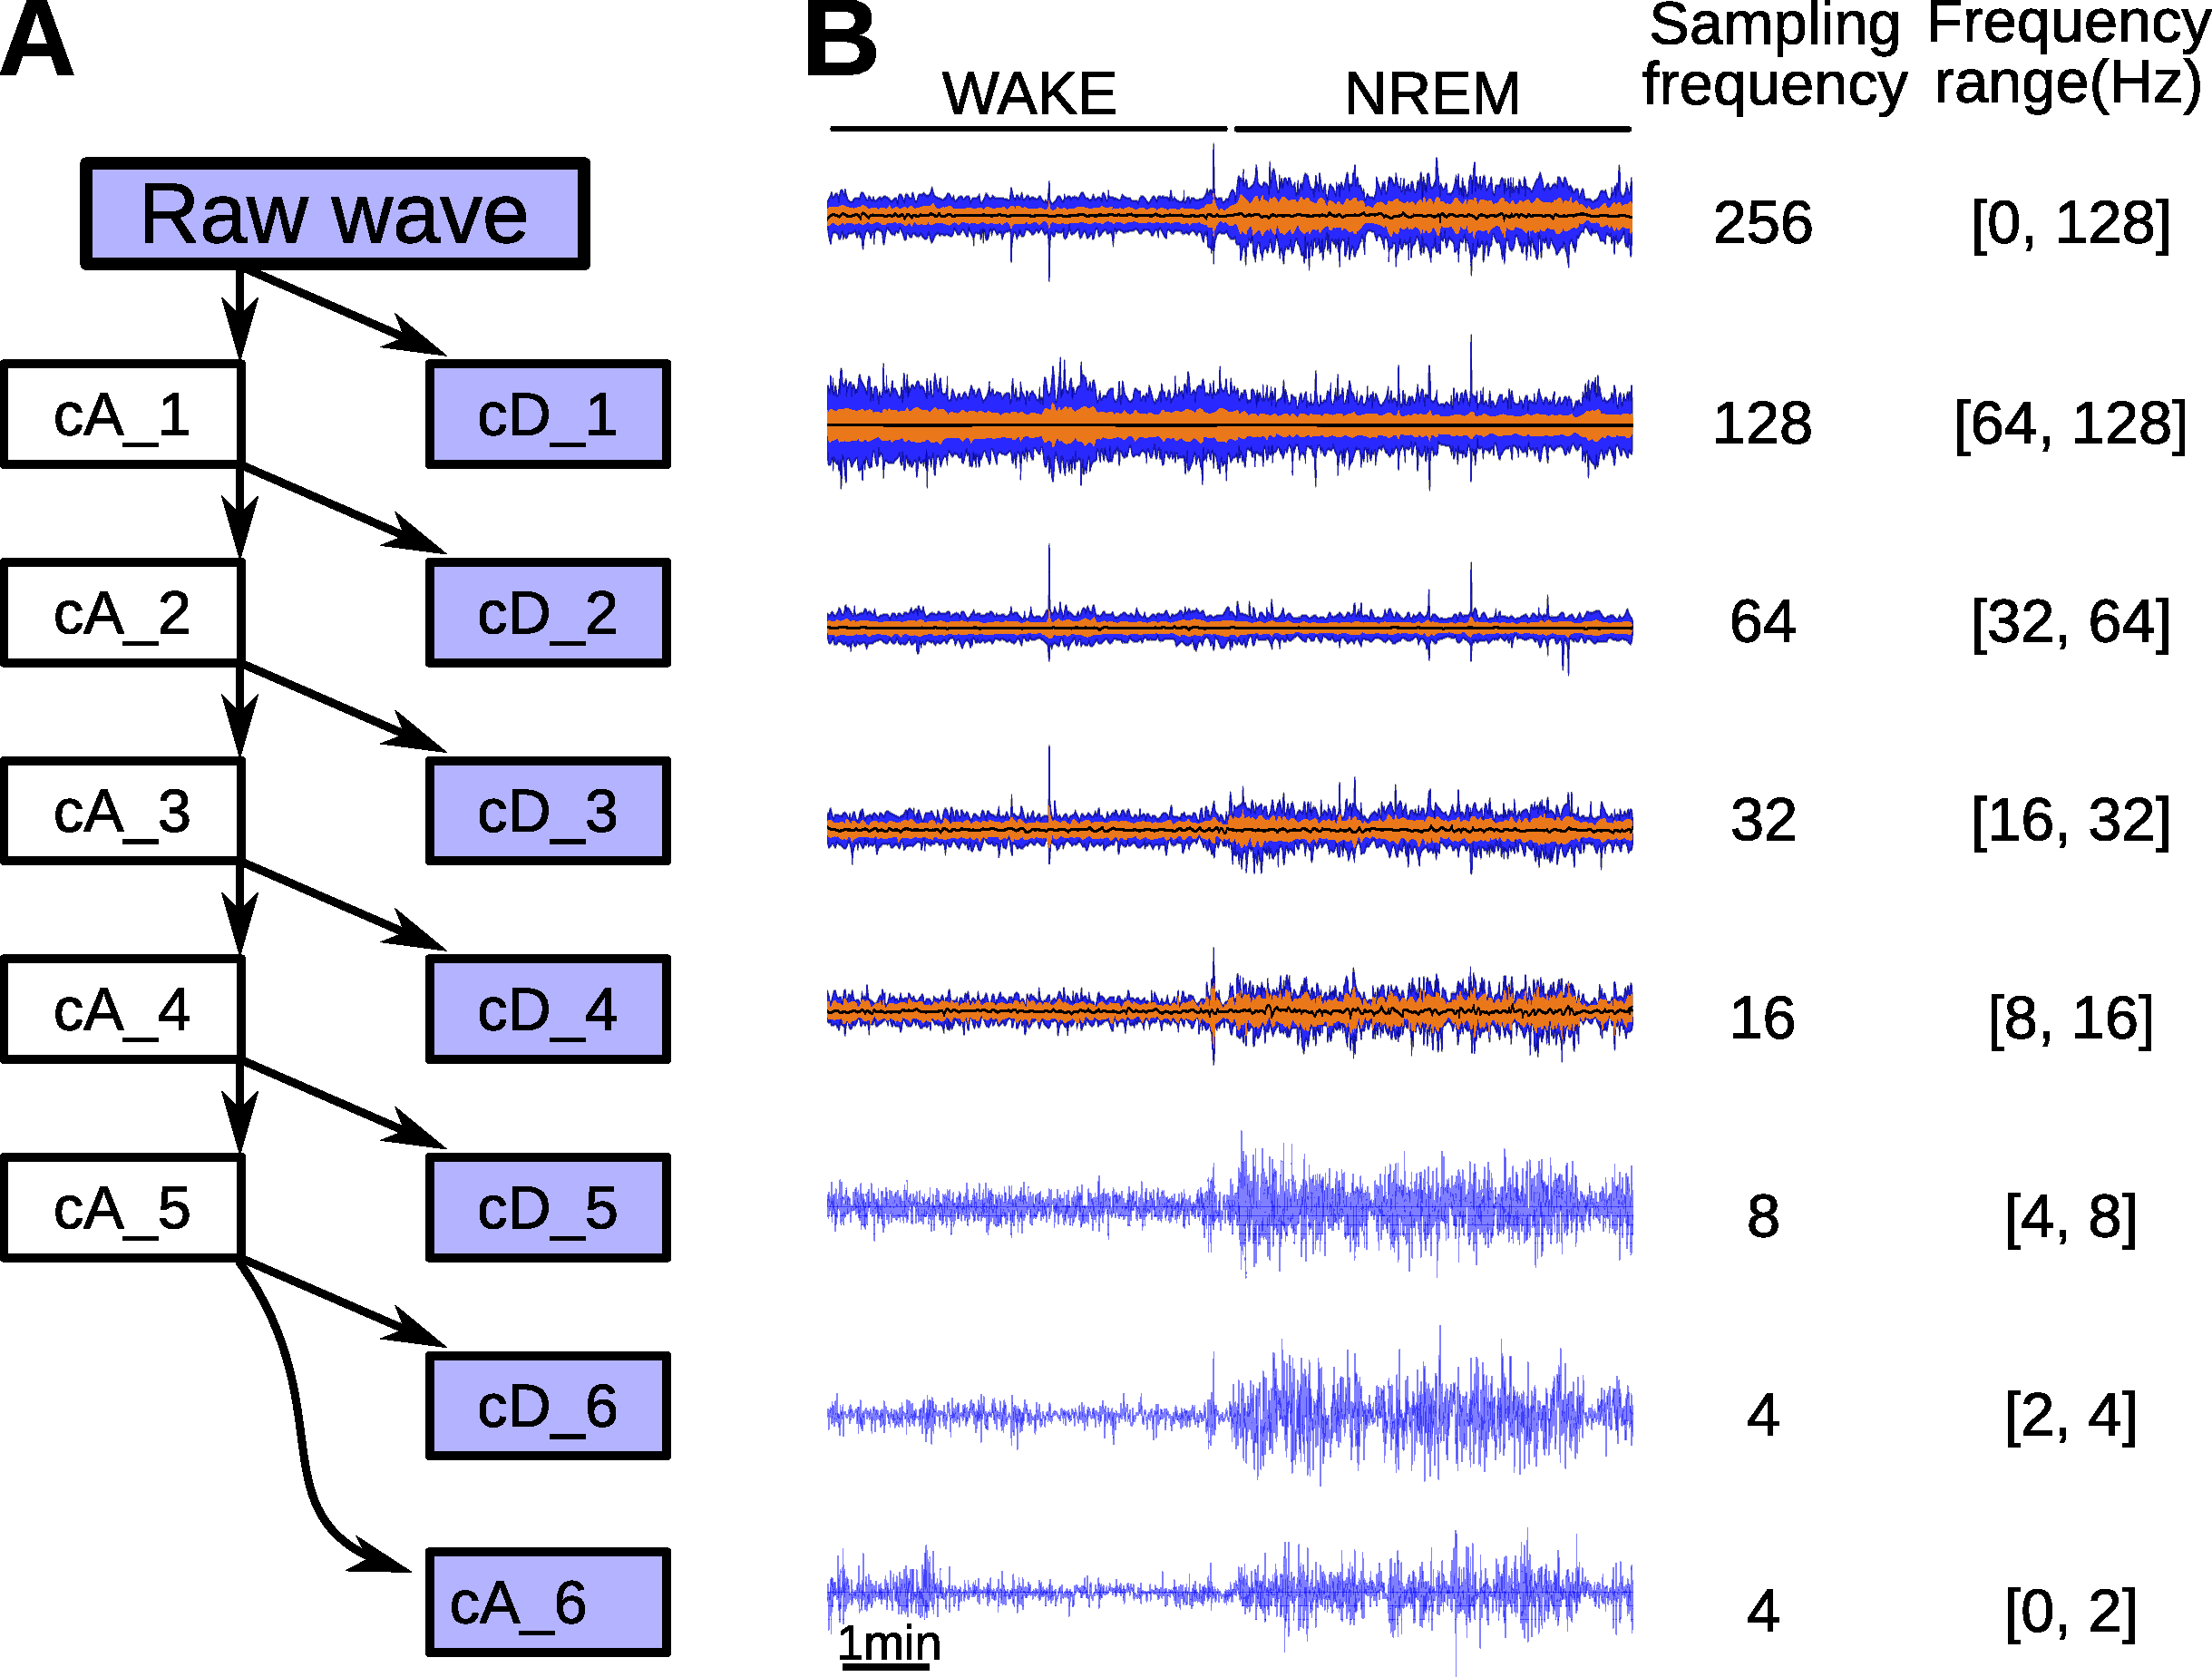
\includegraphics[width=0.95\textwidth]{figures/dwd.pdf}
  \caption{\ctit{Discrete wavelet decomposition.}
	\textbf{A}, Through discrete wavelet transform the initial signal is split into a pair of coefficients: $cA$ and $cD$, which capture the low ($[0, f_s/2]$), and high $[f_s/2, f_s]$ frequency information, respectively.
	Then, discrete wavelet transform is applied iteratively on subsequent $cA$ coefficients ($cA\_1, ..., cA\_n$), thus generating ($cD\_1, ..., cD\_n$).
	In this example, decomposition is performed up to the sixth level ($n=6$).
	\textbf{B}, 
	Ten minutes representing the \gls{eeg} of a transition between a wake and a slow wave sleep(NREM) are shown for the raw
	 wave and for each of the coefficients that are kept for feature extraction (blue rectangles in A).
	 The variation of amplitude in each coefficient corresponds to a concomitant variation of amplitude in the frequency range of this coefficient.
	 In this example, the general increase in power in the raw wave corresponds to an increase of power in the frequency bands below 32Hz, but with a decrease in power above 64Hz.
	%~ Later, each of the eight time series will be segmented into five second epochs, and features are computed for all epochs in the wavelet coefficients and the  raw signal.
	In this figure, the five first signals are too dense to be rendered in a usual fashion. Instead, only local range(blue), inter-quantile range (orange) and median (black line) are represented.
  \label{fig:dwd}
  }
\end{figure}







Importantly, discrete wavelet decomposition was applied \emph{a priory} to the whole signals.
This contrasts with applying decomposition for each epoch \citationneeded{}.
The latter method results in edge effects which would typically need to be attenuated by convolving every epoch with a window function (\eg{} Hamming window).
The maximum decomposition levels for the \gls{eeg} and \gls{emg} signals were six and four, respectively.
Daubechies wavelet, with four vanishing moments (``db4'') was used.

Discrete wavelet decomposition generated seven and five additional time series for \gls{eeg} and \gls{emg}, respectively.
For all 14 time series, a list of 16 features (see table~\ref{tab:features}) was computed in each subsequent non-overlapping five seconds epochs.
Thus, resulting in a total of $p=192$ variables. For each recording ($\simeq 24h$) there were approximately $17000$ epochs.
Some combinations of variables and signals were incalculable.
Therefore, they were removed resulting in an actual number of variables $p=164$.



\begin {table}[!h]
\begin{center}
\caption{\ctit{List of features.}
For clarity, features were classified in four functionnal families.
16 scalar features, in four families, are computed for each epoch.
Since all features are computed for all wavelet coefficients and raw signals (\gls{eeg} and \gls{emg}), a total of 
$16 \times (1+7 + 1 + 3) = 192$ features are generated every five second of recording.
The mathematical detail of the algorithms is provided in the documentation of \pr{} (see appendix).
\label{tab:features}}

\small
\begin{tabular}{|c|c|}
  \hline
  Feature family & features\\
 \hline
 \hline
  Power & \specialcell{\texttt{mean}, \texttt{sd}, \texttt{skewness}, \texttt{kurtosis}\\\texttt{median}, \texttt{min}, \texttt{max}}\\
  \hline
  Hjorth & \texttt{morbidity}, \texttt{complexity}\\
  \hline
  Fractal & \texttt{Petrosian} and \texttt{Higuchi} fractal dimensions\\
  \hline
  Entropy & \specialcell{\texttt{Fisher information}, \texttt{SVD entropy}\\and \texttt{Sample entropy} with $m=2$, and $ r \in \{ 0.2, 1.0, 1.5\}$}\\
 \hline



\end{tabular}
\end{center}
\end{table}



A \py{} package, \pr{}, was developed in order to efficiently
calculate features on heterogeneous time series.
Its complete documentation provided in the appendix of the present document.

\subsection{Addition of temporal features}
In order to integrate temporal information, new variables, depending on past, and future values of predictors, were added for each epochs.
Given a vector $\mathbf{X_t}$ of feature at time $t$,
A first strategy was to define a new vector of feature $\mathbf{{X'}_t}$ as
\begin{equation}
\mathbf{{X'}_t} = \{\mathbf{X_{t-\tau}}, ..., \mathbf{X_t}, ..., \mathbf{X_{t+\tau}}\}
\label{eq:tau}
\end{equation}
with $\tau \in \mathbb{N}$.

Another strategy was to add features representing the local average $\mathbf{W^n_t}$ of each variable over several window sizes $n$.
\begin{equation}
\mathbf{{X'}_t} = \{W^{n_1}_t, W^{n_2}_t, ...\}
\label{eq:window}
\end{equation}
where
\[
\mathbf{W^n_t} = \frac{1}{2n+1} \sum_{i = t-n}^{t+n}{X_i}
\]
and $n$ is a set of odd integers representing window sizes (\eg $\{1,3,7,15\}$).



\subsection{Stratified Cross Validation}
Generally, success of classification of sleep stages is assessed by cross-validation.
In many studies\citationneeded{}, it is implied that cross-validation was performed by making $k$ random training subsets
of the whole data and assessing the model fitted on the remaining subsets (\ie{} k-fold cross-validation).

When working with dense time series (or, for instance, spatial data), it can be suspected that within a statistical block (group),
both features and response variables are very correlated with neighbouring data points.
For instance, the features and label at $t_n$ are expected to be largely similar to the features, and labels at $t_{n+1}$ and $t_{n-1}$.
In statistical terms, $t_{n+1}$ is not independent of $t_{n}$.

If the training sets are drawn completely at random, from a dataset containing multiple long recordings,
the underlying time series would only be made marginally sparser, and the data points missing from
a time series could simply be inferred from the neighbouring points which remain in the training set.

This could give the impression that the model has a very strong predictive power.
However, the goal of cross validation is to assess how well a predictive model would perform on \emph{new data}.
The goal of this study, and most similar studies, was to provide a tool to automatically annotate \emph{new recordings}.
Therefore, it is fairer to perform \emph{stratified cross-validation}, using the different recordings as the stratum levels.
In this study, all cross-validation were performed by training the model with all but one recordings,
and testing it on the recording kept out. This was repeated by successively leaving each recording out.

As shown in figure~\ref{fig:sleep_description}, the prevalence of different states is not balanced. Noticeably, \gls{rem} sleep represents only $10\%$ of all epochs.
This implies that $90\%$ accuracy could be achieved even if all \gls{rem} epoch were misclassified.
For the same reason, the importance of the variables contributing to segregate the minority class (\gls{rem}) could be underestimated.
Therefore, for variable elimination (fig.~\ref{fig:variable_elimination}) and for defining new variables (fig.~\ref{fig:temporal_integration}),
balanced sub-sampled testing sets (750 epochs of each class) were used.

\subsection{Random forests}
Unless specified otherwise, random forests \citationneeded{} were trained with balanced samples of 1000 epochs per class,
50 classification trees and $mtry =\sqrt{p}$.
\texttt{R} software \citationneeded{} was used for prototytping.

In order to enrich every prediction with an associated confidence level, a probabilistic interpretation of random forest was adopted\citationneeded{}.
Then, to produce an overall summary value of confidence, an entropy based metric $c$ was defined as:
\begin{equation}
%~ \[
c = 1 + \frac{1}{log_2(|v|)}\sum{v_i  log_2(v_i)}
%~ \]
\label{eq:entropy}
\end{equation}
where $v_i$ is the proportion of votes for the class $i$. This definition has the property $c \in [0;1]$.

\subsection{Statistics}


\subsection{Performance assessments}
Comparisons of performance between \pr{} and \pyeeg{} were realised by measuring the average (between 2 and 100 run, depending on the algorithm) duration of runtime of algorithms on six
normally distributed ($\mathcal{N}(\mu=0,\sigma=1)$) random time series (\ie white noise) of size $n$,
with $n$ between $256 \times{} 5$ and $256 \times{} 30$.
This was repeated five times for each time series.
For computing  Higuchi fractal dimension, $k_{max}$ was set to $2^3$.
For both approximate entropy and sample entropy, the embedding dimension $m$ was set to $2$, and the distance threshold, $r$, to $1.5$.
For fisher information, the embedding dimension and the delay, $\tau$ were set to $3$ and $2$, respectively.
Finally, spectral entropy was computed for the frequency bands bounded by $\{0, 2^0, 2^1, ..., 2^6\}$Hz, with $f_s = 256.0$.
